\begin{tiny}(gp11)\end{tiny} Mesure algébrique et théorème de Ménéla{\"u}s.\footnote{voir la feuille \href{http://back.maquisdoc.net/data/temptex/fexga.pdf}{Espace affine}(exercices ga04 et ga05.}
\begin{figure}[h!]
  \centering
  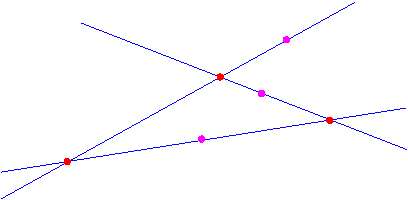
\includegraphics[width=7cm]{Egp11_1.pdf}
  % Egp11_1.pdf: 170x107 px, 72dpi, 6.00x3.77 cm, bb=0 0 170 107
  \caption{Exercice \arabic{enumi}: théorème de Ménéla{\"u}s.}
  \label{fig:Egp11_1}
\end{figure}

\begin{enumerate}
 \item Mesure algèbrique attachée à un vecteur unitaire sur une droite.\\
Soit $\overrightarrow u$ un vecteur directeur unitaire d'une droite $\mathcal D$. Pour tous points $M$ et $N$ de $\mathcal D$, la mesure algébrique $\overline{MN}$ est le nombre défini par :
\begin{displaymath}
 \overrightarrow{MN} = \overline{MN}\overrightarrow{u}
\end{displaymath}
Soient $M'$ et $N'$ deux points distincts de $\mathcal D$, montrer  
\begin{displaymath}
 \overrightarrow{MN} = \dfrac{\overline{MN}}{\overline{M'N'}}\overrightarrow{M'N'}.
\end{displaymath}
\item On considère un vrai triangle $(A,B,C)$ et des points $A'$, $B'$, $C'$ comme sur la figure \ref{fig:Egp11_1}. Les vecteurs $\overrightarrow i$, $\overrightarrow j$, $\overrightarrow k$ sont respectivement directeurs unitaires pour les droites $(AB)$, $(AC)$, $(BC)$.\\ Déterminer à l'aide de mesures algébriques relatives à ces vecteurs les coordonnées des points $A$, $B$, $C$, $A'$, $B'$, $C'$ dans le repère $(A,(\overrightarrow i , \overrightarrow j)$. En déduire le théorème de Ménéla{\"u}s :
\begin{displaymath}
 A' , B', C' \text{ alignés } \Leftrightarrow
\dfrac{\overline{A'B}\,\overline{B'C}\,\overline{C'A}}{\overline{A'C}\,\overline{B'A}\,\overline{C'B}}=1
\end{displaymath}
Pourquoi cette expression est-elle indépendante du choix des vecteurs unitaires ?
\end{enumerate}
